\documentclass[12pt]{article}
\usepackage[english]{babel}
\usepackage[utf8x]{inputenc}
\usepackage{amsmath}
\usepackage{tikz}
\usetikzlibrary{arrows,automata}
\begin{document}

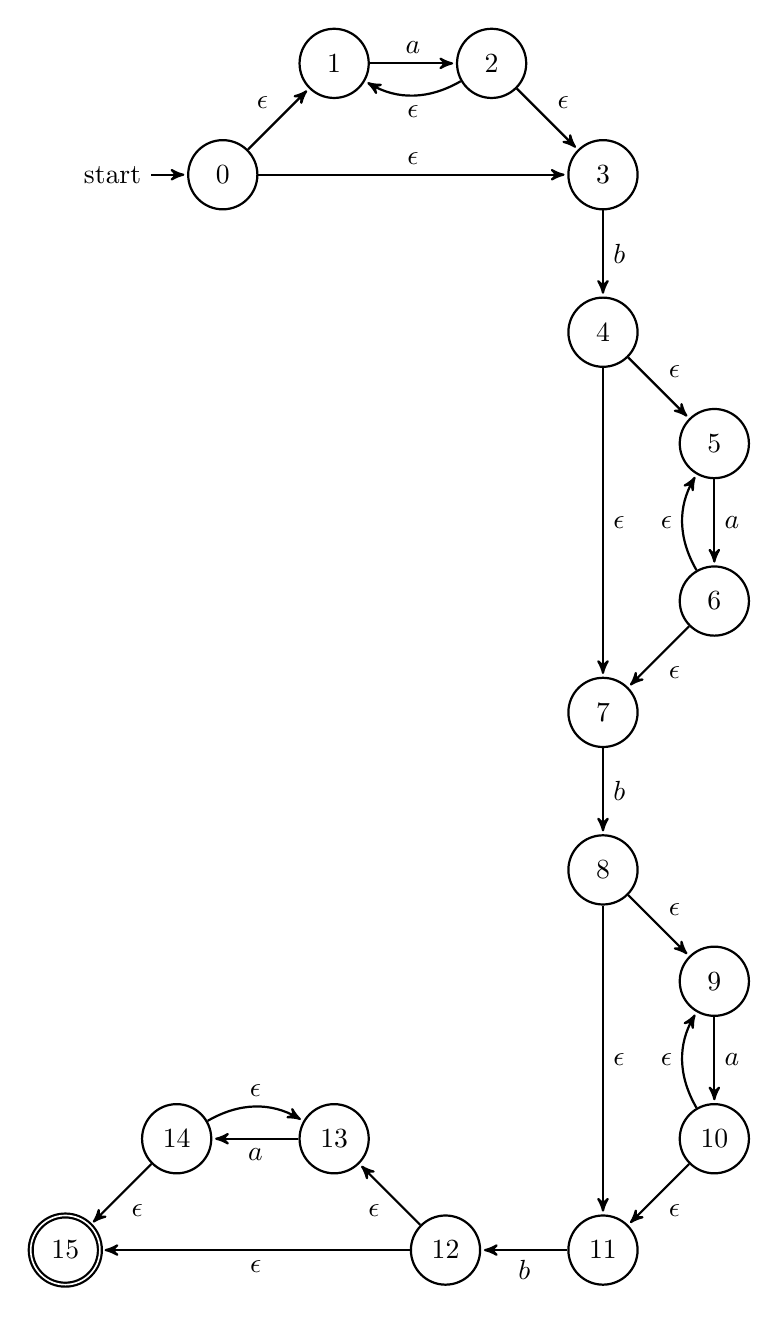
\begin{tikzpicture}[->,>=stealth',shorten >=1pt,auto,node distance=2cm,
    thick,base node/.style={circle,draw,minimum size=8pt}, real node/.style={double,circle,draw,minimum size=17pt}]

  \node[state]          (a){$1$};
  \node[state,initial]  (start) [below left of=a]{$0$};
  \node[state]          (b) [right of=a] {$2$};
  \node[state]  (c)  [below right of=b] {$3$};
  
  \node[state]  (start2) [below of=c]{$4$};
  \node[state]          (a2) [below right of=start2] {$5$};
  \node[state]          (b2) [below of=a2] {$6$};
  \node[state]  (c2)  [below left of=b2] {$7$};

  \node[state]  (start3) [below of=c2]{$8$};
  \node[state]          (a3) [below right of=start3] {$9$};
  \node[state]          (b3) [below of=a3] {$10$};
  \node[state]  (c3)  [below left of=b3] {$11$};
  
  \node[state]  (start4) [left of=c3]{$12$};
  \node[state]          (a4) [above left of=start4] {$13$};
  \node[state]          (b4) [left of=a4] {$14$};
  \node[state,accepting]  (c4)  [below left of=b4] {$15$};
  
  \path (start) edge node {$\epsilon$} (a)
        (a) edge    node {$a$} (b)
        (start) edge node {$\epsilon$} (c)
        (b) edge [bend left] node {$\epsilon$} (a)
        (b) edge      node {$\epsilon$} (c)
        
        
        (start2) edge node {$\epsilon$} (a2)
        (a2) edge    node {$a$} (b2)
        (start2) edge node {$\epsilon$} (c2)
        (b2) edge [bend left] node {$\epsilon$} (a2)
        (b2) edge      node {$\epsilon$} (c2)
        
        (start3) edge node {$\epsilon$} (a3)
        (a3) edge    node {$a$} (b3)
        (start3) edge node {$\epsilon$} (c3)
        (b3) edge [bend left] node {$\epsilon$} (a3)
        (b3) edge      node {$\epsilon$} (c3)
 
        (start4) edge node {$\epsilon$} (a4)
        (a4) edge    node {$a$} (b4)
        (start4) edge node {$\epsilon$} (c4)
        (b4) edge [bend left] node {$\epsilon$} (a4)
        (b4) edge      node {$\epsilon$} (c4)   
        
        (c) edge node {$b$} (start2)
        (c2) edge node {$b$} (start3)
        (c3) edge node {$b$} (start4)
         ;
\end{tikzpicture}
\end{document}